\documentclass{article}
\usepackage{graphicx} % Required for inserting images
\usepackage[utf8]{inputenc}
\usepackage[english]{babel}
\usepackage{amsmath}
\usepackage{amssymb}
\usepackage{amsfonts}
\usepackage{bm}
\usepackage[T1]{fontenc}
\usepackage{geometry}
\geometry{verbose,tmargin=2cm,bmargin=2cm,lmargin=2cm,rmargin=2cm}
\usepackage{orcidlink}

\usepackage{setspace}
\AtBeginDocument{\let~=\nobreakspace}
\spacing{1.5}

\usepackage{lineno}
\linenumbers

\hypersetup{
    unicode=false,          % non-Latin characters in Acrobat's bookmarks
    pdftoolbar=true,        % show Acrobat's toolbar?
    pdfmenubar=true,        % show Acrobat's menu?
    pdffitwindow=false,     % window fit to page when opened
%    pdfstartview={FitW},    % fits the width of the page to the window
    pdftitle={Closed-form Expression of Monero's wallet2 Decoy Selection Algorithm},    % title
    pdfauthor={Rucknium},     % author
    pdfsubject={},   % subject of the document
    pdfcreator={Rucknium},   % creator of the document
    pdfproducer={},  % producer of the document
    pdfkeywords={}, % list of keywords
    pdfnewwindow=true,      % links in new window
    colorlinks=false,       % false: boxed links; true: colored links
    linkcolor=red,          % color of internal links
    citecolor=green,        % color of links to bibliography
    filecolor=magenta,      % color of file links
    urlcolor=cyan           % color of external links
}




\begin{document}

\title{Closed-form Expression of Monero's \texttt{wallet2}\\Decoy Selection Algorithm\\\vspace{.3cm}
\large Draft v0.1\vspace{-.715cm}}
\author{Rucknium\orcidlink{https://orcid.org/0000-0001-5999-8950} }
\date{October 2023}


\maketitle

\section{Modified Log-gamma distribution}

Let $G(x;\alpha,\beta)$ be the Log-gamma cumulative distribution
function (CDF)

\begin{equation}
G(x;\alpha,\beta)=\dfrac{\gamma\left(\alpha,\beta\ln\left(x\right)\right)}{\Gamma\left(\alpha\right)}
\end{equation}

where $\alpha$ is the shape parameter, $\beta$ is the rate parameter,
$\gamma$ is the lower incomplete gamma function, and $\Gamma$ is
the gamma function.

In the \texttt{wallet2} code, $\alpha=19.28$ and $\beta=1.61$. The
$G(x;\alpha,\beta)$ is adjusted in the code to:
\begin{enumerate}
\item Eliminate the portion of the distribution that would be younger than
the youngest spendable output and reallocate it to a uniform distribution
in the \texttt{RECENT\_SPEND\_WINDOW}. The\texttt{ $\frac{x/v_{t}}{1800}\cdot G(1200)$}
term of the expression below performs the reallocation.
\item Re-scale the output index distance unit into seconds. The $x\cdot v_{t}$
term does the re-scaling.
\item Eliminate the portion of the distribution that would be older than
the oldest spendable output and reallocate it to the rest of the distribution.
Terms with $z_{t}$ perform this reallocation.
\end{enumerate}
$G^{*}(x;\alpha,\beta,v_{t},z_{t})$ is the modified CDF that \texttt{wallet2}
uses to randomly generate an output index:

\begin{equation}
G^{*}(x;\alpha,\beta,v_{t},z_{t})=\begin{cases}
0 & \textrm{if }x\cdot v_{t}<0\\
\left(G(x\cdot v_{t}+1200)-G(1200)+\frac{x\cdot v_{t}}{1800}\cdot G(1200)\right)/G\left(z_{t}\cdot v_{t}\right) & \textrm{if }0\leq x\cdot v_{t}\leq1800\\
G\left(x\cdot v_{t}+1200\right)/G\left(z_{t}\cdot v_{t}\right) & \textrm{if }1800<x\cdot v_{t}\leq z_{t}\cdot v_{t}\\
1 & \textrm{if }z_{t}\cdot v_{t}<x\cdot v_{t}
\end{cases}
\end{equation}

$v_{t}$ is the value of \texttt{average\_output\_delay} at the time
$t$ that a specific ring is constructed.

$z_{t}$ is the value of \texttt{num\_usable\_rct\_outputs} at the
time $t$ that a specific ring is constructed.

\section{Counting up unspendable outputs}

Let $\mathcal{U}_{t}$ be the set of outputs at time $t$ that are
not spendable due to custom unlock time or the 60 block lock on coinbase
outputs. Let $u_{t}$ be an element of $\mathcal{U}_{t}$. We need
to find $\mathring{\mathbf{u}}_{t}$, the total the value of the probability
mass function at the unspendable points. The probability mass function
of the spendable outputs must be scaled up by this total so that the
probability mass function sums to one.

Let $u_{t}$ be in block $b_{u_{t}}$. Block $b_{u_{t}}$ contains
outputs with indices $y_{0,u_{t}}$ to $y_{1,u_{t}}$. Therefore,
$y_{0,u_{t}}\leq u_{t}\leq y_{1,u_{t}}$. Note that $y_{0,u_{t}}=u_{t}=y_{1,u_{t}}$
is possible because a block can contain a single output, but no fewer
than one output because every block must have a coinbase transaction
with at least one output. The indices are counted from the first output
in the 11th most recent block, starting from index 1.

\begin{equation}
\mathring{\mathbf{u}}_{t}=\underset{u_{t}\in\mathcal{U}_{t}}{\sum}\dfrac{G^{*}\left(y_{1,u_{t}}+1\right)-G^{*}\left(y_{0,u_{t}}\right)}{y_{1,u_{t}}+1-y_{0,u_{t}}}
\end{equation}


\section{PMF and CDF in closed form}

Let $\mathcal{S}_{t}$ be the set of spendable outputs at time $t$.
Let $s_{t}$ be an element of $\mathcal{S}_{t}$.

Let $s_{t}$ be in block $b_{s_{t}}$. Block $b_{s_{t}}$ contains
outputs with indices $y_{0,s_{t}}$ to $y_{1,s_{t}}$. Therefore,
$y_{0,s_{t}}\leq s_{t}\leq y_{1,s_{t}}$. Note that $y_{0,s_{t}}=s_{t}=y_{1,s_{t}}$
is possible. The probability mass function of the \texttt{wallet2}
decoy selection algorithm is 

\begin{equation}
f(s_{t})=\dfrac{G^{*}\left(y_{1,s_{t}}+1\right)-G^{*}\left(y_{0,s_{t}}\right)}{y_{1,s_{t}}+1-y_{0,s_{t}}}\cdot\dfrac{1}{1-\mathring{\mathbf{u}}_{t}}
\end{equation}

The CDF can be found by computing the cumulative sum of the PMF of
spendable outputs:

\begin{equation}
F(s_{t})=\underset{i\in\mathcal{S}_{t}\textrm{ s.t. }i\leq s_{t}}{\sum}\dfrac{G^{*}\left(y_{1,i}+1\right)-G^{*}\left(y_{0,i}\right)}{y_{1,i}+1-y_{0,i}}\cdot\dfrac{1}{1-\mathring{\mathbf{u}}_{t}}
\end{equation}


\section{Example}

Below is the PMF for rings in transactions that were constructed and
broadcast between the 2,999,999th and 3,000,000th block, which would
have been included in the 3,000,000 block in usual circumstances.
Just the first 5,000 outputs are shown.

\begin{figure}
    \centering
    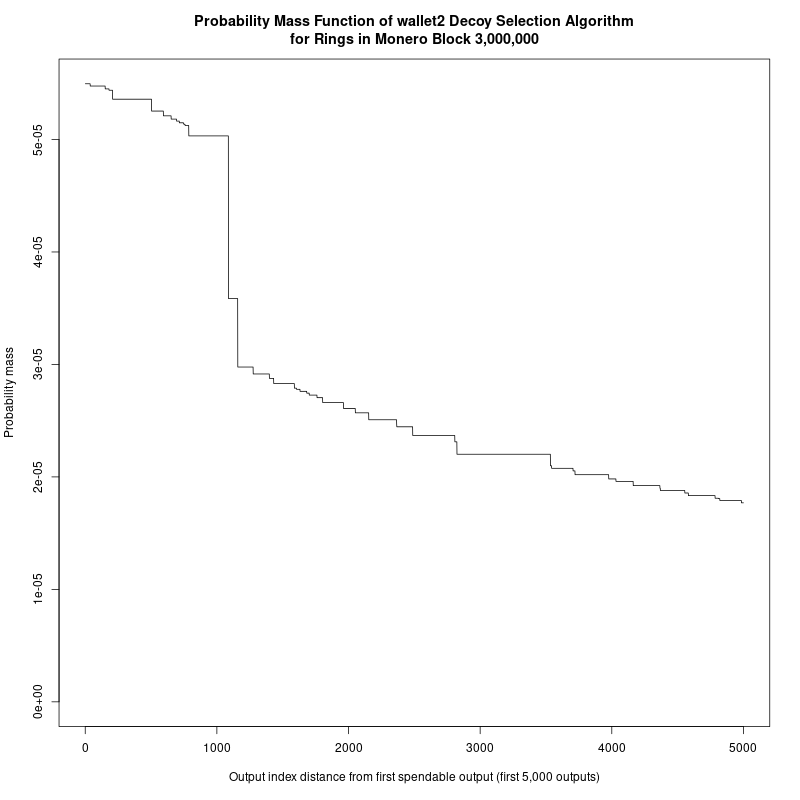
\includegraphics[width=1\linewidth]{images/wallet2-DSA-plot-draft.png}
    \caption{Example PMF}
    \label{fig:enter-label}
\end{figure}

\end{document}
